\documentclass[conference]{IEEEtran}
\IEEEoverridecommandlockouts





%%%%%%%%%%%%%%%%%%%%%%%%%
%%%% LATEX PACKAGES %%%%%
%%%%%%%%%%%%%%%%%%%%%%%%%

\usepackage{amsmath,amssymb,amsfonts}
\usepackage{algorithmic}
\usepackage{graphicx}
\usepackage[font=small]{caption}
\usepackage[font=footnotesize]{subcaption}
\usepackage{textcomp}
\usepackage{xcolor}
\usepackage{hyperref}
\usepackage{svg}
\usepackage{enumitem}
\usepackage[backend=biber,
            %style=apa,
            %style=numeric,
            style=numeric-comp,
            bibstyle=numeric,
            %citestyle=authoryear-comp,
            citestyle=numeric-comp,
            %sorting=nyt,
            sorting=none,
            maxnames=8,
            minnames=3
            %maxcitenames=2,
            %mincitenames=1
            ]{biblatex}

\usepackage{easyReview} % use to help review the paper (https://ctan.org/pkg/easyreview)





%%%%%%%%%%%%%%%%%%%%%%%%%%%%
%%%%% USER DEFINITIONS %%%%%
%%%%%%%%%%%%%%%%%%%%%%%%%%%%

\addbibresource{references.bib}

\def\BibTeX{{\rm B\kern-.05em{\sc i\kern-.025em b}\kern-.08em
    T\kern-.1667em\lower.7ex\hbox{E}\kern-.125emX}}

\newcommand{\orcid}[1]{\href{https://orcid.org/#1}{
\includegraphics[height=1em]{figures/orcid.pdf}}}

\newcommand{\etal}{\textit{et.~al.}}





\begin{document}





%%%%%%%%%%%%%%%%%
%%%%% TITLE %%%%%
%%%%%%%%%%%%%%%%%

\title{System Framework for the\\Robot@Factory 4.0 Competition\\
\thanks{This work is financed by National Funds through the Portuguese funding agency, FCT -- Fundação para a Ciência e a Tecnologia, within project LA/P/0063/2020
(DOI: \href{https://doi.org/10.54499/LA/P/0063/2020}{10.54499/LA/P/0063/2020}).}}





%%%%%%%%%%%%%%%%%%%%%%%%%%%%%%%%%%%%%%%%%%%%%%
%%%%% AUTHORS + AFFILIATIONS INFORMATION %%%%%
%%%%%%%%%%%%%%%%%%%%%%%%%%%%%%%%%%%%%%%%%%%%%%

\author{%
\IEEEauthorblockN{%
Ricardo B. Sousa\IEEEauthorrefmark{1}\IEEEauthorrefmark{2}~\orcid{0000-0003-4537-5095},
Cl\'{a}udia D. Rocha\IEEEauthorrefmark{2}\IEEEauthorrefmark{3}~\orcid{0000-0001-7254-0346},
Jo\~{a}o G. Martins\IEEEauthorrefmark{1}\IEEEauthorrefmark{2}~\orcid{0000-0002-6567-4802},
Jo\~{a}o Pedro Costa\IEEEauthorrefmark{1},\\
Jo\~{a}o Tom\'{a}s Padr\~{a}o\IEEEauthorrefmark{1},
Jos\'{e} Maria Sarmento\IEEEauthorrefmark{2}\IEEEauthorrefmark{3}~\orcid{0000-0002-4332-9645},
Jos\'{e} Pedro Carvalho\IEEEauthorrefmark{1}\IEEEauthorrefmark{4}~\orcid{0009-0008-3416-5694},
Maria S. Lopes\IEEEauthorrefmark{1}\IEEEauthorrefmark{2}~\orcid{0009-0001-7216-2469},\\
Paulo G. Costa\IEEEauthorrefmark{1}\IEEEauthorrefmark{2}~\orcid{0000-0002-4846-271X},
Ant\'{o}nio Paulo Moreira\IEEEauthorrefmark{1}\IEEEauthorrefmark{2}~\orcid{0000-0001-8573-3147}}
%
\IEEEauthorblockA{%
\IEEEauthorrefmark{1}Faculty of Engineering, University of Porto (FEUP), 4200-465 Porto, Portugal\\
Email: \texttt{up\{\href{mailto:up201503004@edu.fe.up.pt}{201503004},%
\href{mailto:up201806222@edu.fe.up.pt}{201806222},%
\href{mailto:up201806431@edu.fe.up.pt}{201806431},%
\href{mailto:up202108766@edu.fe.up.pt}{202108766},%
\href{mailto:up201806775@edu.fe.up.pt}{201806775}\}@edu.fe.up.pt}\\
\texttt{\{\href{mailto:jpcarvalho@fe.up.pt}{jpcarvalho},%
\href{mailto:paco@fe.up.pt}{paco},%
\href{mailto:amoreira@fe.up.pt}{amoreira}\}@fe.up.pt}%
}
\IEEEauthorblockA{%
\IEEEauthorrefmark{2}CRIIS -- Centre for Robotics in Industry and Intelligent Systems\\
INESC TEC -- Institute for Systems and Computer Engineering, Technology and Science, 4200-465 Porto, Portugal\\
Email: \texttt{\{\href{mailto:claudia.d.rocha@inesctec.pt}{claudia.d.rocha},%
\href{mailto:jose.m.sarmento@inesctec.pt}{jose.m.sarmento}\}@inesctec.pt}%
}
\IEEEauthorblockA{%
\IEEEauthorrefmark{3}School of Science and Technology\\
University of Tr\'{a}s-os-Montes and Alto Douro (UTAD), 5000-801 Vila Real, Portugal%
}
\IEEEauthorblockA{%
\IEEEauthorrefmark{4}C2SR -- Cyber-Physical Control Systems and Robotics\\
SYSTEC -- Research Center for Systems and Technologies, 4200-465 Porto, Portugal%
}
}





\maketitle





%%%%%%%%%%%%%%%%%%%%%%%%%%%%%%%
%%%%% ABSTRACT + KEYWORDS %%%%%
%%%%%%%%%%%%%%%%%%%%%%%%%%%%%%%

\begin{abstract}
Robotic competitions stand as platforms to propel the forefront of robotics research while nurturing STEM education, serving as hubs of both applied research and scientific innovation.
In Portugal, the Portuguese Robotics Open~(FNR) is a national event with several robotic competitions, including the Robot@Factory~4.0 competition.
This competition presents an example of deploying autonomous robots on a factory shop floor.
Although the literature has works proposing system frameworks for the original version of the Robot@Factory competition, none of them proposes a system framework for the Robot@Factory~4.0 version that presents the hardware, firmware, and software to complete the competition and achieve autonomous navigation.
So, this paper proposes a complete system framework for the Robot@Factory~4.0 competition that is modular and open-access, enabling future participants to use and improve it in future editions.
This work is the culmination of all the knowledge acquired by winning two editions of the competition.
\end{abstract}

\begin{IEEEkeywords}
autonomous mobile robots, robot competitions, robot at factory 4.0
\end{IEEEkeywords}





%%%%%%%%%%%%%%%%%%%%%%%%%%%%
%%%%% DOCUMENTION BODY %%%%%
%%%%%%%%%%%%%%%%%%%%%%%%%%%%

\section{Introduction}\label{sec:intro}

Since 1997, the RoboCup\footnote{\label{note:robocup}\url{https://www.robocup.org/}} federation has organised international robot soccer competitions, including Small and Middle Size League (SSL and MSL, respectively) robots and humanoids, and more recently, competitions focused on service (RoboCup@Home) and industrial (RoboCup@Work) autonomous robots.
Another example is the Formula Student\footnote{\url{https://www.imeche.org/events/formula-student}} competition, which has been held in Europe since 1999. This event includes several categories (combustion, electric, hybrid, and driverless autonomous systems) while being an educational engineering platform in several fields, such as robotics, computer science, mechanical, and electrical and computer engineering.
More recently, the F1TENTH~\cite{literature:competitions:f1tenth} and the Indy Autonomous Challenge~(IAC)~\cite{literature:competitions:indy} were created to push further the research on autonomous systems and also serve as STEM education platforms for students.

In Portugal, the Portuguese Robotics Open~(FNR)\footnote{\label{note:fnr}\url{https://www.festivalnacionalrobotica.pt/}} is an event hosting several competitions divided into major and junior categories.
These competitions include qualification events to decide the Portuguese teams participating in the RoboCup, international championships, autonomous driving, dragster, and the Robot@Factory Lite and Robot@Factory~4.0 competitions, which are more oriented to industrial cases.
In particular, the Robot@Factory~4.0 competition aims to represent the deployment of autonomous mobile robots on a factory shop floor. The robots should be able to transport materials between warehouses or machines that process those materials, considering the robots' ability to self-localise and navigate in order to avoid collisions with the walls.

The current literature has works oriented toward the original and present versions of the Robot@Factory competition hosted at FNR (Robot@Factory and Robot@Factory~4.0, respectively).
Ribeiro~\etal~\cite{literature:ratf:ribeiro-2017} presented their design and development path towards the robot used to participate in the original version of the competition.
The robot was a three-wheeled omnidirectional robot with five processing units (including a Raspberry Pi 2 Model B and two Arduino Mini), a 2D laser scanner, and an Inertial Measurement Unit (IMU) used to obtain a pose estimation.
Similarly, Pinto~\etal~\cite{literature:ratf:pinto-2023} also proposed a three-wheeled omnidirectional robot to participate in the original competition.
The proposed framework used wheeled odometry and 2D laser data to estimate the robot pose with the PerfectMatch~\cite{literature:ratf:pinto-2023:perfect-match} algorithm, while only using a single processing unit, namely, a Raspberry Pi 3.
Finally, Braun~\etal~\cite{literature:ratf:braun-2024} presented the development of a four-wheeled mecanum platform specifically designed for the Robot@Factory~4.0 competition, with a Raspberry Pi 4 and an Arduino Mega 2560 as processing units. 
This work focused on the mechanical design and electronics of the robot, including the description of the sensory perception system composed by a camera and a 2D laser scanner.
In conclusion, the works of Ribeiro~\etal~\cite{literature:ratf:ribeiro-2017} and Pinto~\etal~\cite{literature:ratf:pinto-2023} are not intended for the present version of the Robot@Factory competition, while the work of Braun~\etal~\cite{literature:ratf:braun-2024} does not cover the software architecture and implementation part of the robot.

Thus, this paper proposes a modular and open-access system framework for an autonomous robot to be able to participate in future editions of the Robot@Factory~4.0 competition.
The description of the proposed framework includes the hardware, firmware, and software implemented by the 5dpo Robotics Team\footnote{\url{https://5dpo.github.io/}} that led the team to win two consecutive editions of the competition.
All the code relative to firmware and software developed within the context of the competition, 3D models of the robot parts, and additional documentation are available in a public GitHub repository\footnote{\label{note:repo}\url{https://github.com/5dpo/5dpo_ratf_2023}}.
Indeed, this repository containing the implementation of the proposed framework may be used by future participants in the competition to have an initial start on their development and push it even further to foster their STEM education knowledge.
To the best of the authors' knowledge, and according to the related works information found in the literature, no framework encompasses hardware, software, and system integration to allow building an entire robot system for the Robot@Factory~4.0 competition.


The remaining of this paper is organised as follows.
Section~\ref{sec:ratf} presents a brief summary of the current version of the Robot@Factory 4.0 competition.
Section~\ref{sec:system} describes the architecture of the proposed system framework.
Then, Sections~\ref{sec:hw}, \ref{sec:fw}, and \ref{sec:sw} characterise the hardware, firmware, and software implemented and used in the competition, respectively.
Section~\ref{sec:tests} presents the results originated from the participation in two editions of Robot@Factory~4.0.
Lastly, Section~\ref{sec:conclusions} formulates the final conclusions and future work.





\section{Robot@Factory 4.0 Competition}\label{sec:ratf}

The competition presents the problem of deploying autonomous mobile robots on a factory shop floor (illustrated in Figure~\ref{fig:ratf:track-2023}).
One or more robots should transport materials between warehouses or machines, depending on the type of materials received in the input warehouse.
The robots will transport three different parts from the incoming warehouse: blue, green, and red boxes.
The first is considered a final part; thus, it is sent directly to the output warehouse.
The second one is an intermediate part that must receive a transformation to a blue box at either machines A or B.
Lastly, the red box must suffer two transformations, first on machine A to a green part, and then on B to a blue box.
Furthermore, the competition is divided into three rounds. The rounds are distinguished by the type of parts received in the incoming warehouse: only blue parts are considered in the first round, in the second one may exist some green parts (usually, two boxes), and in the third round may have both green and red parts (usually, two and one boxes, respectively).
The robot must communicate with a Wi-Fi server to get which part types are available for each slot in the incoming warehouse at the start of each run.

\begin{figure}[!t]
\centering
\centerline{\includesvg[height=0.7\columnwidth]{figures/ratf-track_2023.svg}}
\caption[Shop floor of the Robot@Factory 4.0 2023 edition composed by warehouses (input on the top-left and output on the bottom-right of the floor), machines (middle wall markings, where the machines A are on the left and B on the right side), and ArUco markers.]{Shop floor of the Robot@Factory 4.0 2023 edition composed by warehouses (input on the top-left and output on the bottom-right of the floor), machines (middle wall markings, where the machines A are on the left and B on the right side), and ArUco markers~\cite{ratf:github-repo}.}
\label{fig:ratf:track-2023}
\end{figure}

As for the robot design, each robot must fit into a $30\times30$~cm rectangle with a maximum height of 30~cm.
The robot must be completely autonomous and cannot communication with any type of external systems that are not provided by the organisation.
Unlike the original version of the Robot@Factory competition, the shop floor has no guiding lines nor outer walls delimiting the shop floor area.
The teams can use the ArUco markers on the floor for localisation (the guidelines of the competition available in \cite{ratf:github-repo} present the ground-truth position of those).
Additionally, the teams can place their own markers (e.g., reflectors or poles) near the corners of the factory, providing that these do not exceed an occupied area of $10\times 10$~cm and a maximum height of 50~cm.

In terms of the final classification, the team with the highest total number of parts correctly transported to the outgoing warehouse or to a machine is the winner.
In case of teams with the same total number of points, the first criteria is the number of correctly places parts in the outgoing warehouse, and the second criteria is the shortest time to finish the round.





\section{System Architecture}\label{sec:system}

The system framework proposed in this paper and illustrated in Figure~\ref{fig:system-architecture} is composed of three elements: all the components and mechanics related to the robot (motors, sensors, actuators), the firmware layer to interact with low-level devices (including motors speed reading and control) running in an Arduino~Mega~2560, and the software executing in a Raspberry~Pi~4B~4G (drivers to interact with the firmware and other devices, localisation and navigation modules).
First, the robot is a four-wheeled omnidirectional platform designed in the scope of the Robot@Factory~4.0 competition, using a 3D printer to make the parts of the platform. The robot includes a switch and a solenoid to sense and transport the boxes.
Next, the firmware layer controls the motors' angular speed, counts the encoder quadrature pulses, reads the switch state, and actuates the solenoid according to the software.
Then, the software executes Robot Operating System~(ROS) nodes implemented in C++ to interact with the firmware and other devices (including the 2D laser scanner), estimate the robot pose, provide a Human-Machine Interface~(HMI) interface based on \texttt{rviz}, and enable the autonomous navigation of the robot to execute the desired tasks.
The following sections explain each element of the system framework in depth.

\begin{figure}[!t]
\centering
\centerline{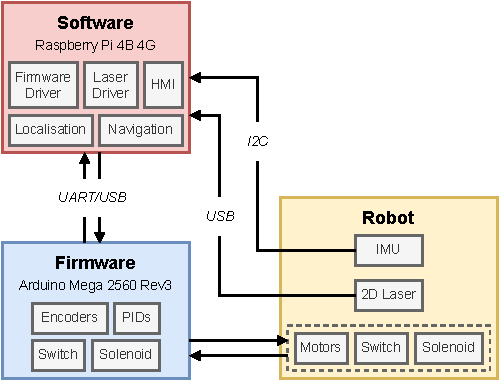
\includegraphics[width=0.8\columnwidth]{figures/system-architecture.pdf}}
\caption{System architecture proposed in this paper for the Robot@Factory~4.0 competition.}
\label{fig:system-architecture}
\end{figure}





\section{Hardware}\label{sec:hw}

\subsection{Robot motion}

In terms of the robot motion, the four-wheeled omnidirectional platform designed in the scope of the competition is illustrated in Figure~\ref{fig:robot}.
This platform uses 60~mm aluminium mecanum wheels, where the distance between the front-back and left-right wheels is 0.152~m and 0.193~m, respectively.
As a consequence of using four mecanum wheels, the robot has holonomic kinematics, originating that the robot's linear and angular velocities are decoupled from each other (e.g., the robot can manoeuvre around obstacles without affecting the orientation)~\cite{book:intro-robotics}.
Indeed, this design choice results in an increased flexibility in terms of path planning and trajectory control, where the robot may rotate along the trajectory without requiring to do on-the-spot rotations.

\begin{figure}[!t]
\centering
\subfloat[][]{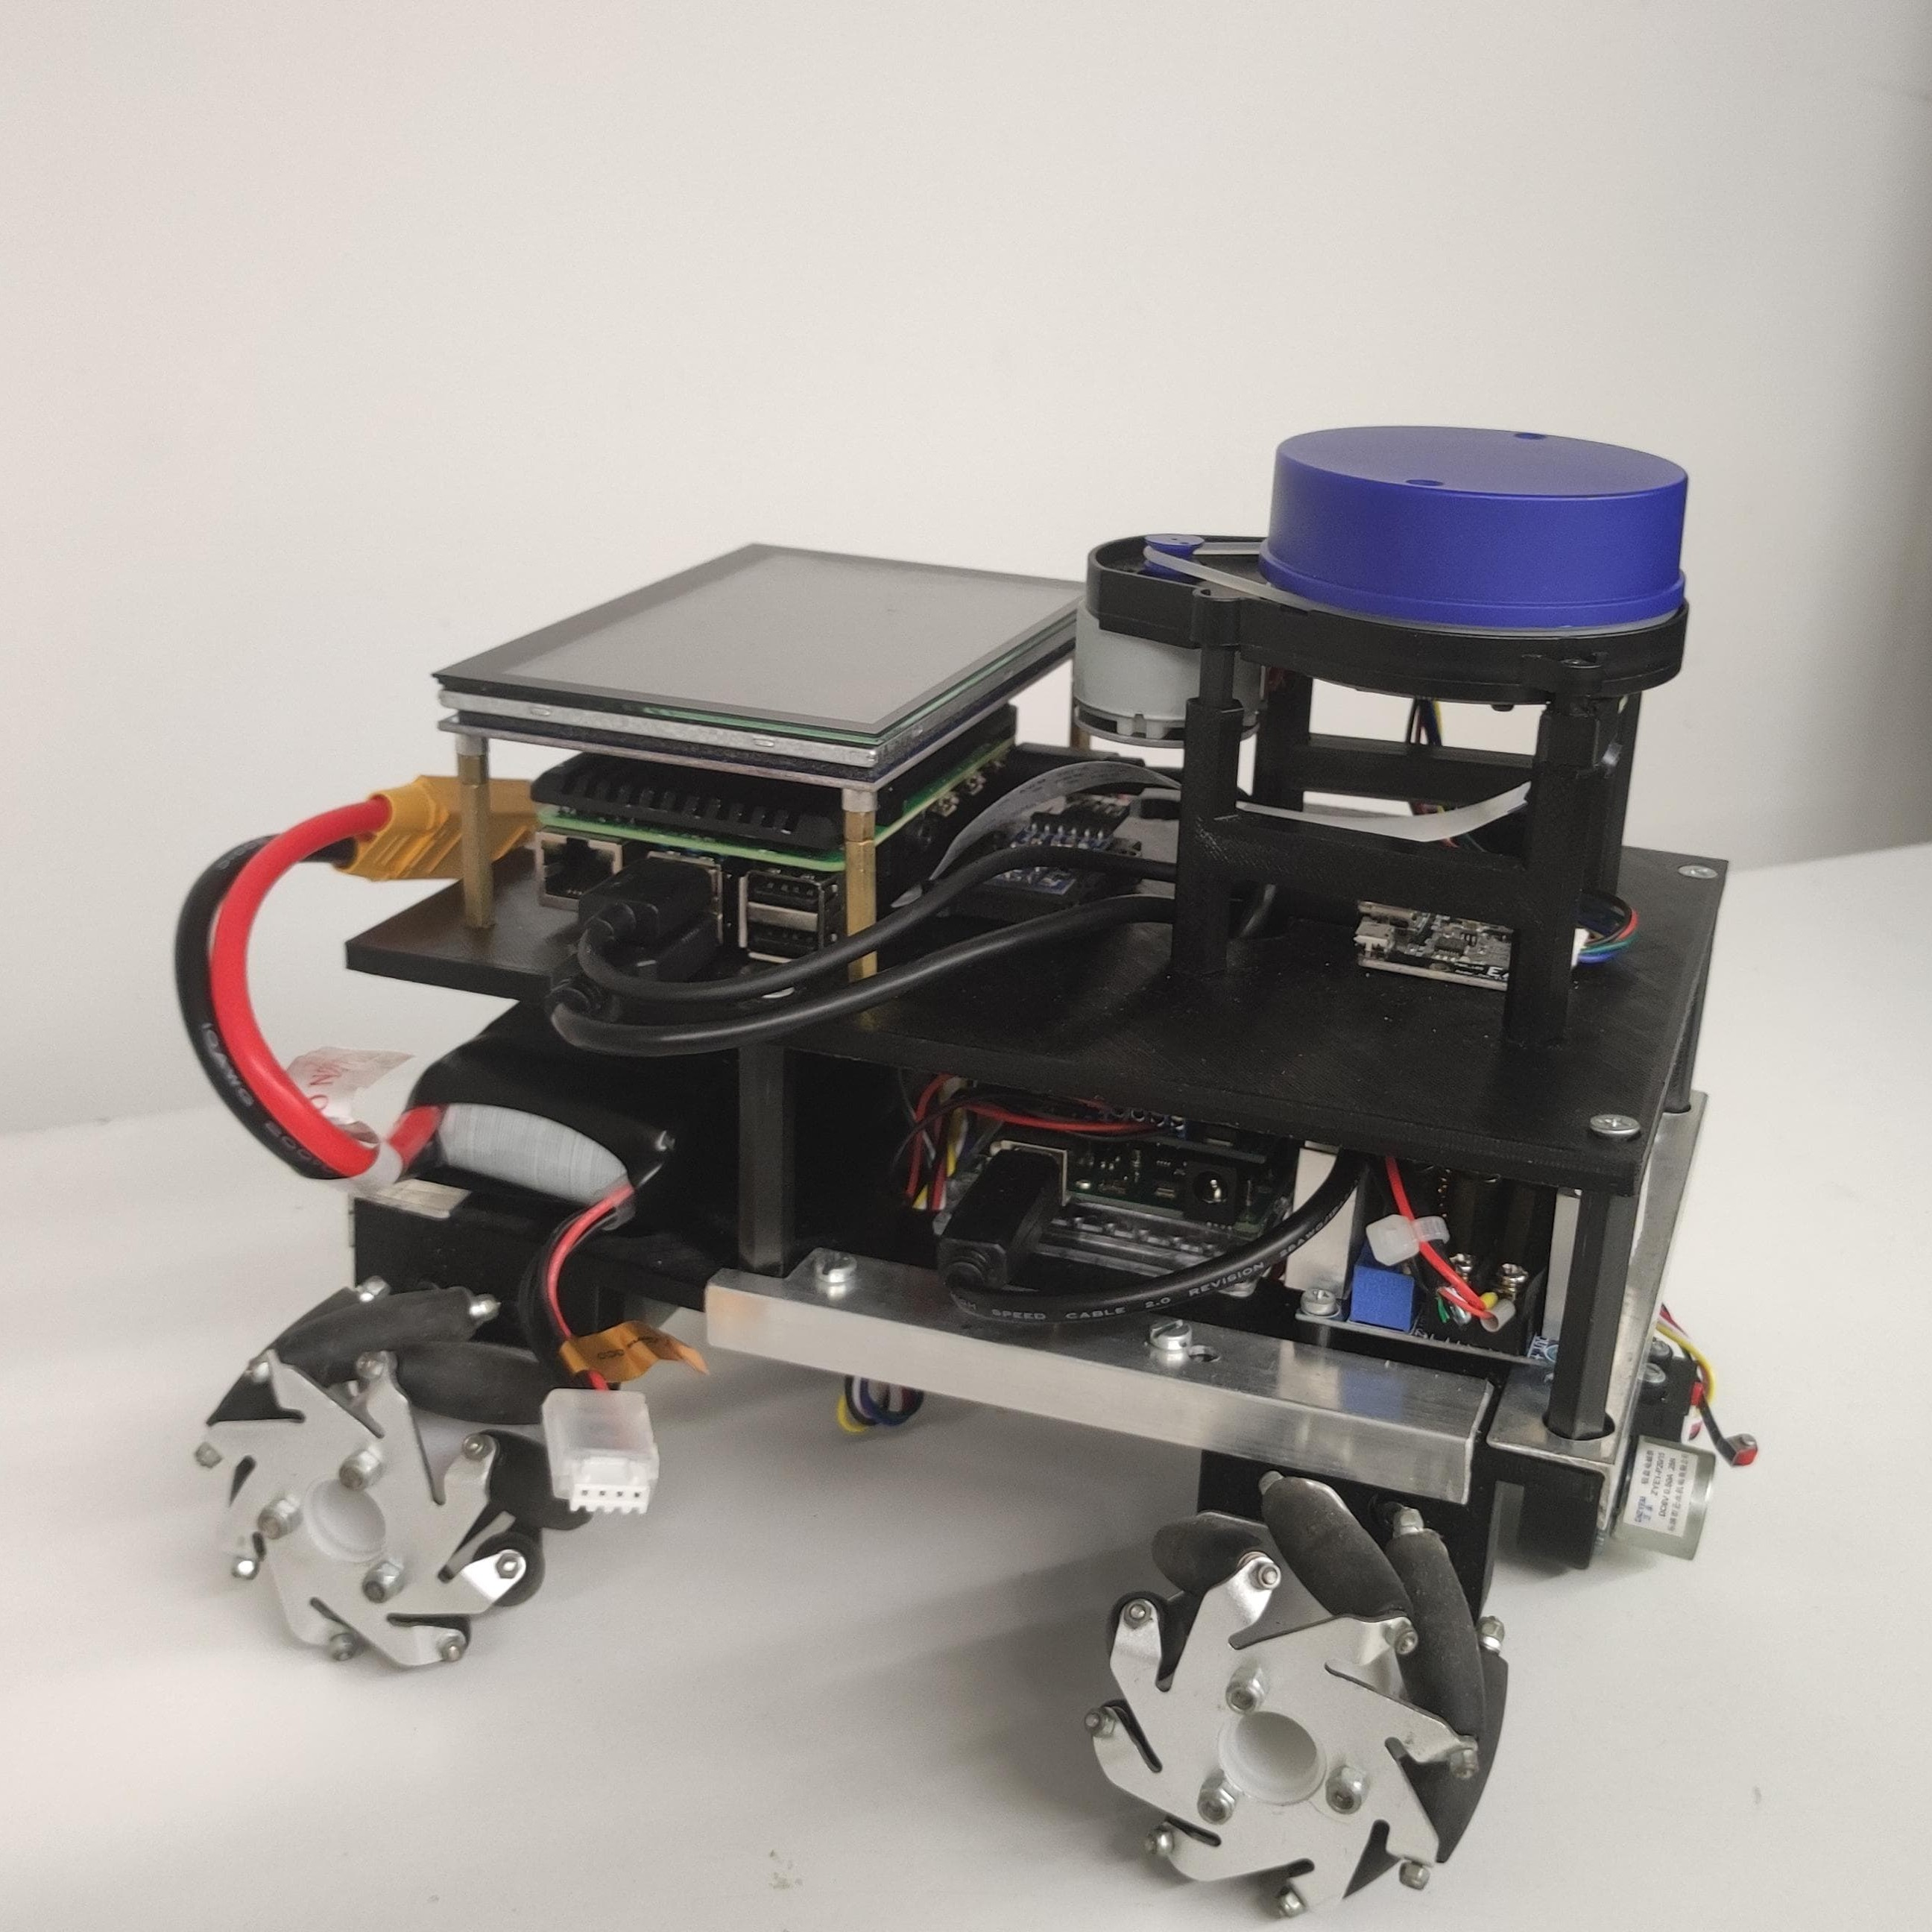
\includegraphics[width=0.6\columnwidth]{figures/robot-perspective.jpeg}%
\label{fig:robot:cool-pic}}
\linebreak
\subfloat[][]{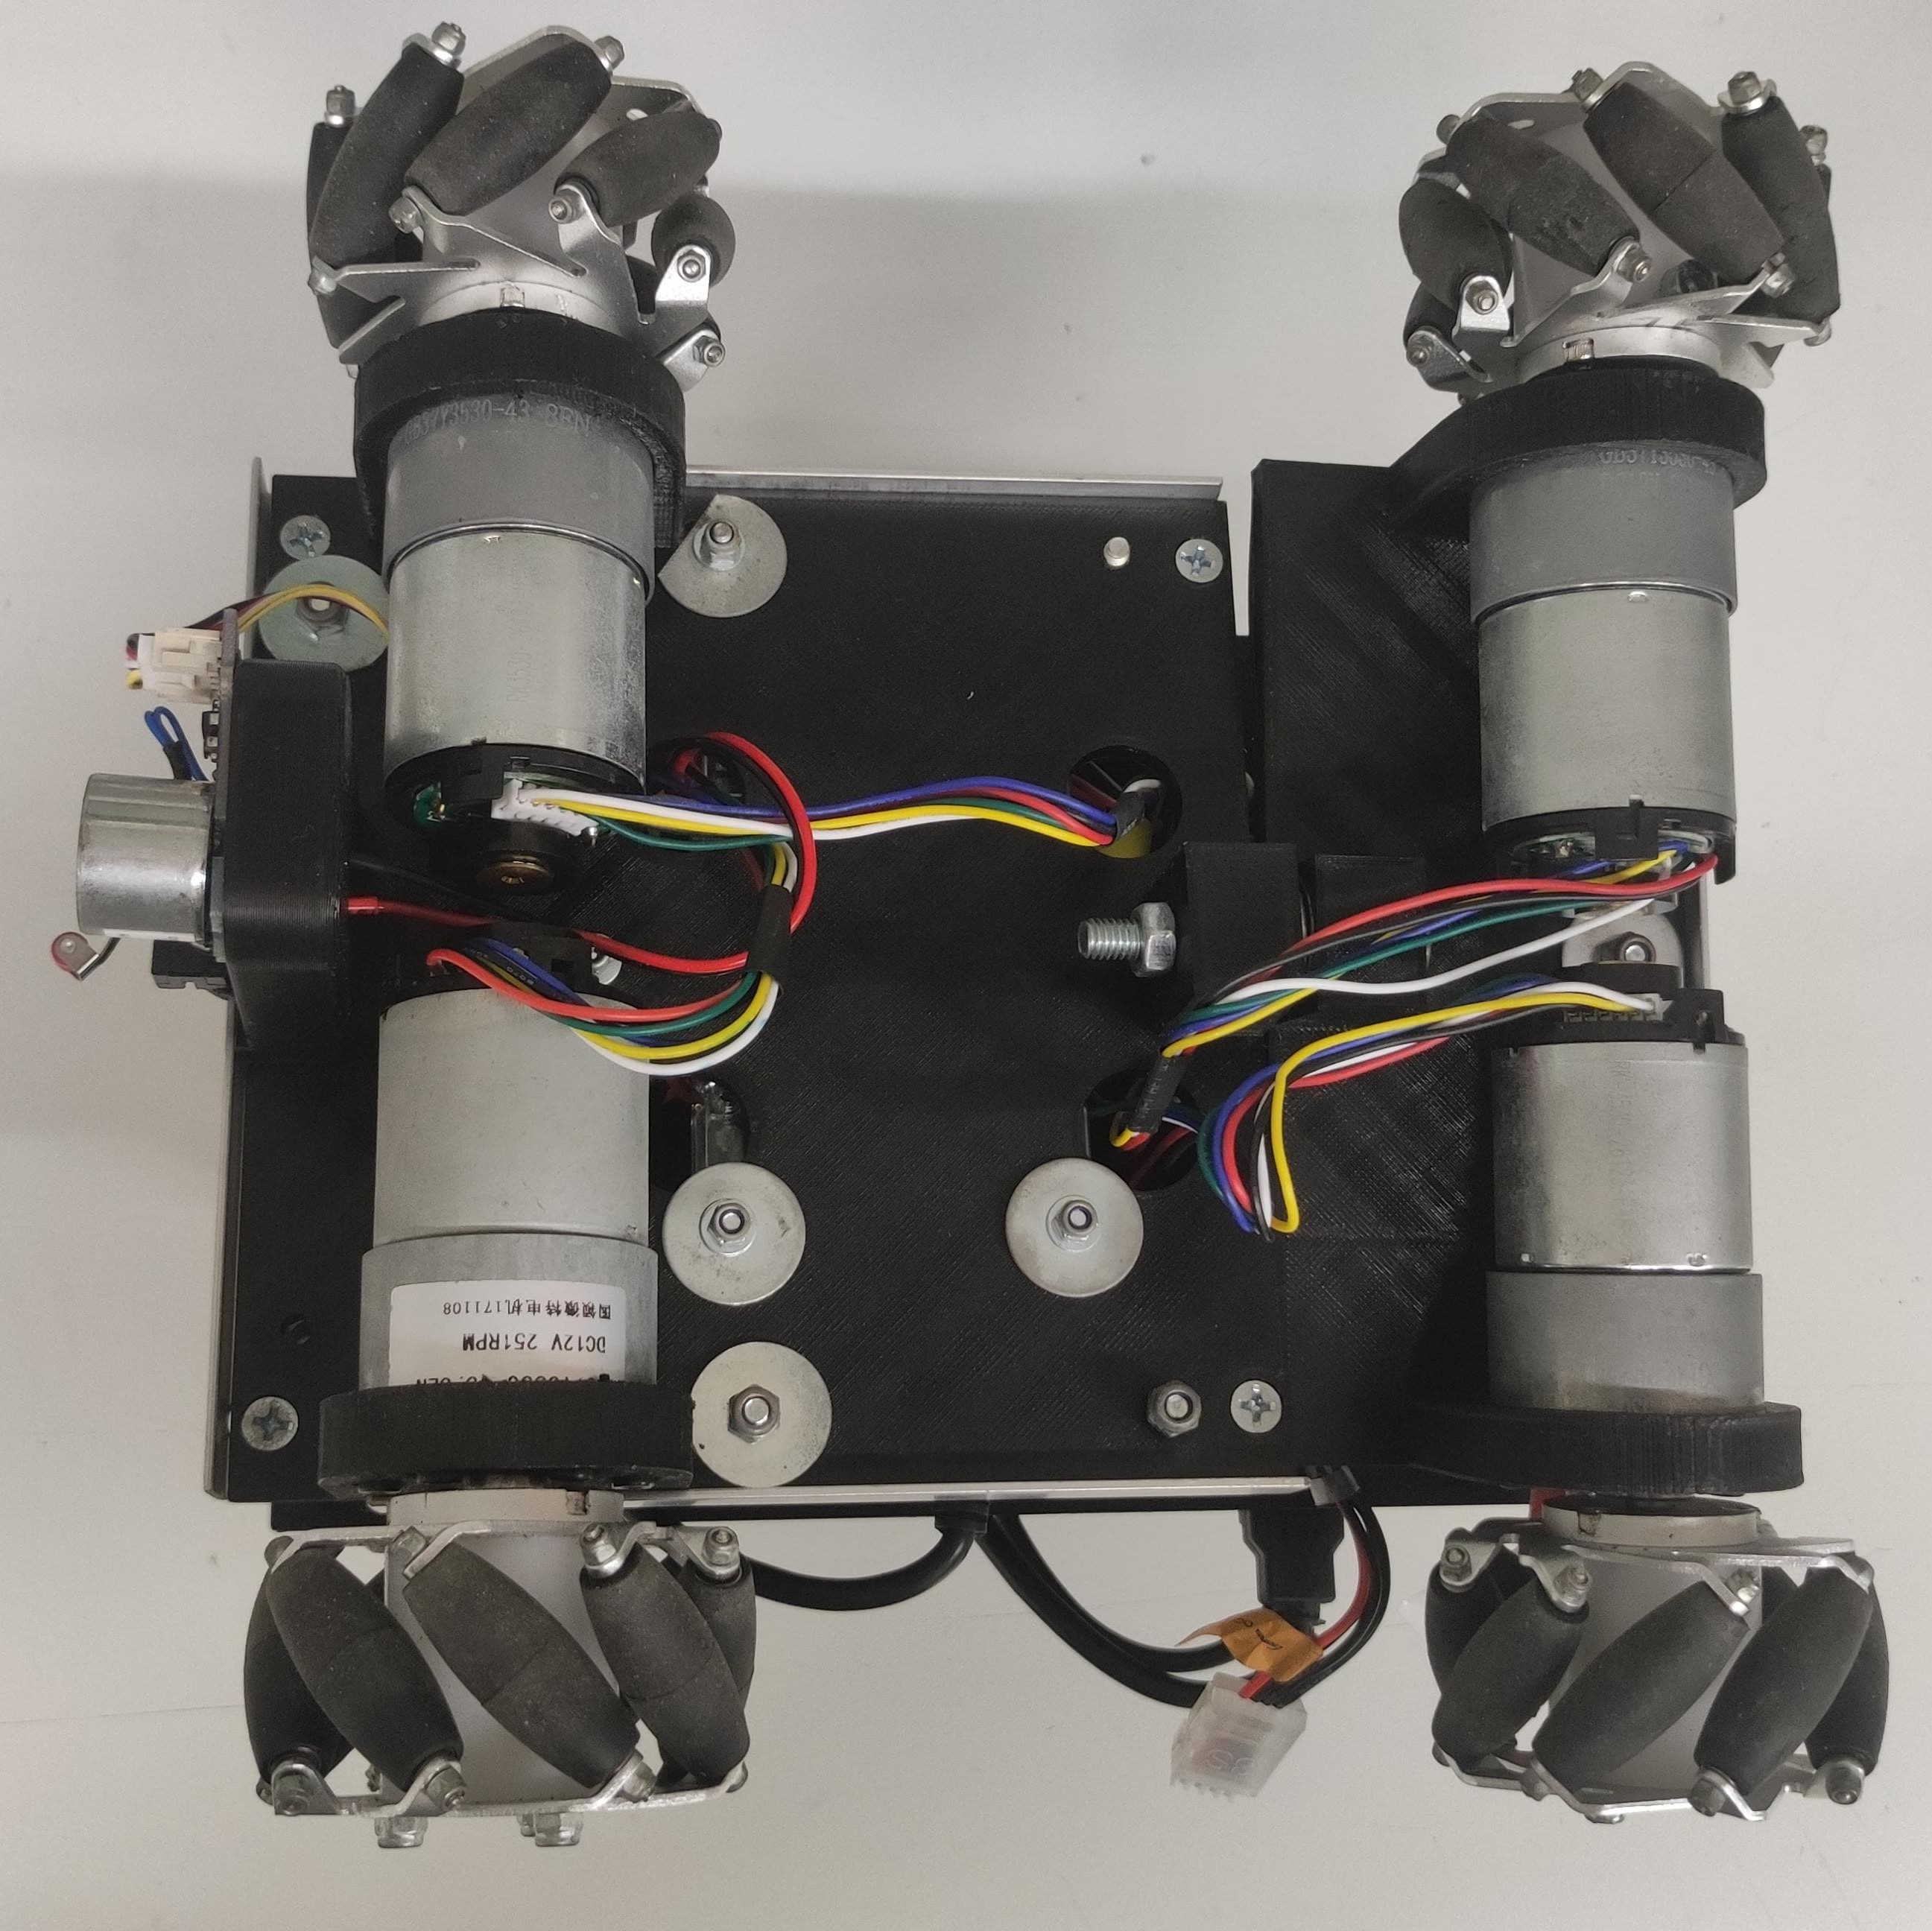
\includegraphics[width=0.6\columnwidth]{figures/robot-bottom.jpeg}%
\label{fig:robot:suspension}}
\caption{Four-wheeled omnidirectional platform designed in the scope of the competition:
(a) the robot;
(b) the bottom with the suspension.}
\label{fig:robot}
\end{figure}

Furthermore, the motors chosen are 12V~DC motors with 251~rpm at no load from DFRobot.
The motors include a 43.7:1 metal gearbox and integrated quadrature encoders based on the Hall effect.
These encoders have a resolution of 16 counts per revolution of the motor shaft, resulting in approximately 700~counts of the gearbox's output shaft.
If the firmware can process the pulses, this setup results in a resolution of 2800~pulses per revolution on the robot's wheels.

An additional design constraint must be accounted for because the robot has four wheels.
Conventionally, the static stability of a robot requires a minimum of three wheels, where the triangle formed by the ground contact points must contain the centre of gravity. The latter is ensured in the proposed platform by most of the components being in the volume between the front and back wheels.
However, once the number of contact points exceeds three, the geometry requires some form of flexible suspension on uneven terrain~\cite{book:intro-robotics}.
Even though the floor of the competition should be flat and even, Figure~\ref{fig:robot:suspension} shows the suspension put in the robot to be compatible with terrain with minor imperfections in terms of its flatness.



\subsection{Processing unit}

Next, an Arduino Mega 2560 executes the firmware described in this paper. This microcontroller board is compatible with several open-source libraries, including the SPI\footnote{\href{https://www.arduino.cc/reference/en/language/functions/communication/spi/}{https://www.arduino.cc/reference/en/language/functions/communication/\\spi/}} (communication with SPI devices) and TimerOne~\&~TimerThree\footnote{\label{note:timers-lib}\url{https://www.pjrc.com/teensy/td_libs_TimerOne.html}} (implementation of timers with PWM pins) libraries used in this work.
Moreover, the 5V operating voltage of the Arduino~Mega is directly compatible with the voltage of the encoders of the motors and the electromagnet actuation.

As for the software, the Raspberry~Pi~4B~4GB executes all the ROS nodes implemented in C++.
Given that this paper uses ROS 1 Noetic, the Operating System~(OS) running in the Raspberry Pi was the Raspberry OS (Legacy) based on Debian Buster.
However, the OS Ubuntu~20.04 may also be used instead of Raspbian, in case there is no need for graphical output.
Also, the advantages of using Raspberry~Pi are its compatibility with the Raspberry~Pi Camera module (e.g., for ArUco markers detection) and its 40 General-Purpose Input/Output~(GPIO) pins compatible with SPI and I2C devices.



\subsection{Sensors}

In terms of the sensory system on the robot, in addition to the wheel odometry data obtained from the encoders, the robot is equipped with a 2D laser scanner and an IMU.
The first is a YDLIDAR~X4 based on the principle of triangulation.
This laser has a 360º Field-of-View~(FoV), a range between 0.12~m and 10~m, and a typical scanning frequency and angle resolution of 7~Hz (using the device interface to connect and power up the laser through a USB connection) and 0.5º, respectively.
Considering the maximum area of $1.7\times1.2$~m for the shop floor defined in the competition rules, the sensor is considerably suitable for this application.
However, other alternatives based on Time-of-Flight~(ToF) technologies, such as the DTOF~LD19 and RPLIDAR~S2 lasers, may provide more precise distance data.
As for the IMU, the sensor employed on the robot is the Waveshare 10 Degrees-of-Freedom~(DoF).
This IMU is a low-cost sensor with an accelerometer, magnetometer, gyroscope, and temperature sensor.
However, only the accelerometer and gyroscope data are used in the scope of this paper. The data communication between IMU and Raspberry~Pi is through an I2C bus.

Even though camera data is not used in this paper, the four-wheeled omnidirectional platform illustrated in Figure~\ref{fig:robot} is also equipped with an RGB Raspberry Pi Camera Board v2.
This camera has a sensor with 8MP and a resolution of up to 1080p.
The main advantages of using this camera are its ribbon cable compatibility with the CSI port on the Raspberry Pi, native drivers for the camera in the Raspberry Pi, and compatibility with the OpenCV computer vision library.



\subsection{Electronics}

As for powering up the robot, the platform has a Gens Ace 5000mAh battery with a 3S cell configuration and an 11.1V nominal voltage.
The battery directly powers the wheels' motors and the Arduino~Mega.
Although 
Furthermore, a 300W DC/DC buck converter compatible with the conversion from 6--40V in the input to 1.2--36V in the output (maximum of 20A) creates a second voltage rail of 5V.
This rail powers up the Raspberry~Pi~4B and the electromagnet.
Although it would be advisable to have a voltage regulator between the battery and the other components, the approach taken in the platform simplifies as much as possible the electronics of the system.

Moreover, the Raspberry Pi powers up the 2D laser scanner and the IMU through the USB connection and the GPIO interface, respectively.
In order to control the motors' angular speed, the system must have an electronic board able to generate PWM signals for the motors.
Thus, the Arduino~Mega used in the platform also has the Adafruit Motor Shield.
This shield allows to drive up to four DC motors, communicating with the microcontroller over I2C.



\subsection{3D modelling}

Lastly, all the parts composing the structure of the omnidirectional platform are 3D printed in PLA.
These parts are available in STEP files in the public repository\footref{note:repo}.
The leading software used to design the parts was originally the OpenSCAD open-source modeller, and then, the team transitioned to AutoDesk~Fusion~360.
The latter has both free personal and academic licenses available for use.
Even so, STEP files are compatible with other 3D modelling software such as FreeCAD and SolidWorks, allowing to use other programs to perform modifications in the original parts.





\section{Firmware}\label{sec:fw}

The robot's firmware is implemented in the Arduino Mega 2560 as a PlatformIO project (the latter has extensions for both CLion and Visual Studio Code).
This firmware includes counting the encoders' pulses, angular speed control of the motors, the serial communication with the Raspberry~Pi through a UART/USB connection, and the simple logic associated with reading the switch state and actuating the solenoid.



\subsection{Wheel encoders}

First, relative to counting the encoders' pulses, Figure~\ref{fig:fw:encoders} illustrates the quadrature inherently related to a two-channel (A and B) encoder.
Considering that the logical values of the two channels are known for the current time instant $k$ and the previous instant $k-1$,  there are 16 possible possibilities for all possible logic values of the last and current states of the two channels (presented in Table~\ref{tab:fw:encoders}).
Thus, the firmware developed for the framework proposed in this paper employs a lookup table to speed up the encoders' reading, being to attach an interruption to read the channels' logic values at 50~kHz.
This periodic interruption is implemented using the TimerOne library\footref{note:timers-lib}.
Even though other boards, such as the Raspberry Pi Pico and the Teensy ones, have programmable input/output machines that may improve even further the frequency of checking the channels and counting the pulses (avoiding skipping pulses due to higher angular speeds of the motors), the Arduino Mega does not offer that possibility.


\begin{figure}[!t]
\centering
\centerline{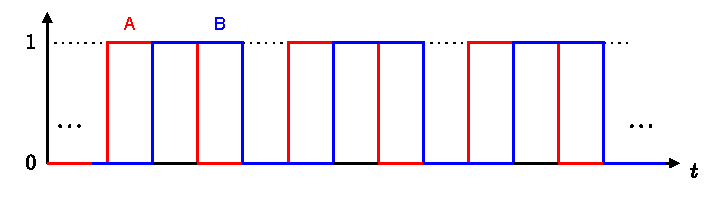
\includegraphics[width=0.8\columnwidth]{figures/encoders.pdf}}
\caption{Encoders signals example.}
\label{fig:fw:encoders}
\end{figure}

\begin{table}[t!]

\centering
\caption{Lookup Table of the Possible Values for the Previous ($k-1$) and Current ($k$) State on each Channel A and B, and the corresponding Increment on the Pulses Counters ($\Delta_k$).}
\label{tab:fw:encoders}



\begin{tabular}{c c | c c | c}

%% HEADER
\hline
\textbf{$\text{A}_{k-1}$} &
\textbf{$\text{B}_{k-1}$} &
\textbf{$\text{A}_{k}$} &
\textbf{$\text{B}_{k}$} &
\textbf{$\Delta_{k}$}\\
\hline



%% TABLE CONTENTS
0 & 0 & 0 & 0 &  0\\ % maintains state (stopped)
0 & 0 & 0 & 1 & -1\\
0 & 0 & 1 & 0 &  1\\
0 & 0 & 1 & 1 &  0\\ % not valid state (skipped transition)
\hline
0 & 1 & 0 & 0 &  1\\
0 & 1 & 0 & 1 &  0\\ % maintains state (stopped)
0 & 1 & 1 & 0 &  0\\ % not valid state (skipped transition)
0 & 1 & 1 & 1 & -1\\
\hline
1 & 0 & 0 & 0 & -1\\
1 & 0 & 0 & 1 &  0\\ % not valid state (skipped transition)
1 & 0 & 1 & 0 &  0\\ % maintains state (stopped)
1 & 0 & 1 & 1 &  1\\
\hline
1 & 1 & 0 & 0 &  0\\ % not valid state (skipped transition)
1 & 1 & 0 & 1 &  1\\
1 & 1 & 1 & 0 & -1\\
1 & 1 & 1 & 1 &  0\\ % maintains state (stopped)
\hline



\end{tabular}



\end{table}


Furthermore, there are two occasions in Table~\ref{tab:fw:encoders} where the delta of the pulse counters is~0.
One of them is when the previous state is maintained in the current instant, meaning that the wheel did not move.
The other situation is when a transition in the quadrature of the encoders is skipped, e.g., having the previous state $\{A,B\}_{k-1}={0,0}$ and the current one $\{A,B\}_{k}={1,1}$.
This situation does not reveal the wheel's direction, thus setting the delta to 0 to avoid counting erroneous pulses.

Regarding the resolution of counting the encoders' pulses, as stated in Section~\ref{sec:hw}, the encoders in the omnidirectional platform have a resolution of 16~counts per revolution on the motors' shaft.
The approach implemented in this paper can process the quadrature of the encoders, quadrupling the resolution.
Consequently, the final resolution obtained in the firmware is~64 and 2796.8~pulses per revolution on the motors' shaft and at the wheels, respectively (the latter considering the 43.7 reduction ratio in the motors' gears). This final resolution corresponds to 0.128º/pulse at the wheel.



\subsection{Wheel angular speed control}

The control of the motors' angular speed is similar to the methodology presented in Sousa~\etal~\cite{5dpo:sousa-2021}.
Proportional-Integrative~(PI) controllers set the motors' input voltage. Considering that the motors have a dead zone, a Hammerstein nonlinear block is used to compensate for the existence of that zone.
Then, the windup effect is compensated by limiting the voltage computed from the PI controllers and the Hammerstein block to the maximum value supported by the motors.
When the voltage exceeds these limits, the integration part of the PI controller remains unchanged.
Given that PWM signals can be used to control the DC motors, these signals are directly handled by the Adafruit Motor Shield with a frequency of 1.6~KHz (the maximum value allowed by the shield).
The communication between the shield and the Arduino Mega is through an SPI connection.



\subsection{Serial communication}

As for exchanging data between the firmware and the software modules, this data transmission is handled over a serial communication between the Raspberry~Pi and the Arduino~Mega.
The serial port's baud rate is 115200~bps, which is considered a safe setup in terms of timing errors.

The channels library\footnote{\url{https://github.com/P33a/MeArmControlVarSpeed}} manages the data protocol for the communication.
This paper employs the version that puts the hexadecimal representation of the data as ASCII characters in the communication stream.
Indeed, the data frame of this version is as follows: the first byte is a plain letter in ASCII format representing a channel, and the following 8 bytes are the hexadecimal representation of 4-byte data packets as ASCII characters (0--9, A--F).
The channel's letter can be any letter between a--z and G--Z.
Even though the channel's library has a binary form to compact the data part of the frame from 8 to 4~bytes, being more efficient, plain ASCII greatly facilitates the debugging of the firmware data streams by using a simple serial monitor.
Thus, the channels configuration used in the firmware is the following one:
\begin{itemize}[nosep]
\item Arduino Mega $\rightarrow$ Raspberry Pi:
  \begin{itemize}[nosep]
  \item \texttt{g}: pulse count of the back-right wheel (ticks)
  \item \texttt{h}: pulse count of the back-left wheel (ticks)
  \item \texttt{i}: pulse count of the front-right wheel (ticks)
  \item \texttt{j}: pulse count of the front-left wheel (ticks)
  \item \texttt{k}: interval time between control cycles (us)
  \item \texttt{r}: reset signal
  \item \texttt{s}: switch signal
  \end{itemize}
\item Raspberry Pi $\rightarrow$ Arduino Mega:
  \begin{itemize}[nosep]
  \item \texttt{G}: reference speed of the back-right wheel (rad/s)
  \item \texttt{H}: reference speed of the back-left wheel (rad/s)
  \item \texttt{I}: reference speed of the front-right wheel (rad/s)
  \item \texttt{J}: reference speed of the front-left wheel (rad/s)
  \item \texttt{K}: PWM value of the motors:
    \begin{itemize}[nosep]
    \item (value $>>$ 24) \& 0x03: motor index (0..3)
    \item (value) \& 0xFFFF: PWM value (0..max)
    \end{itemize}
  \item \texttt{L}: solenoid actuation
  \end{itemize}
\end{itemize}

This configuration allows the communication of the encoders' pulse counters, the desired angular speed for the motors, and the switch and solenoid signals required to interact and transport the boxes between locations between the two processing units in the omnidirectional platform.
The interval time is to monitor the control of the angular speed control and the reset signal to reinitialise the firmware driver in the software.
Additionally, channel \texttt{K} is to actuate the PWM directly (and so, being able to set the voltage of the motors), allowing a possible automatic calibration of the PI parameters using the software to set the voltage of the motors and logging the angular speed after processing the rate of pulses per second read from the encoders.



\section{Software}\label{sec:sw}

In terms of the software components of the system framework, all the software is developed in C++ and ROS~1~Noetic and is executed in the Raspberry Pi 4B 4GB.
The software includes the drivers developed in the scope of the competition, the robot localisation estimation and its integration with the laser scanner, wheeled and inertial odometry, autonomous navigation through the shop floor, and the HMI interface.



\subsection{Drivers}

As previously mentioned in Section~\ref{sec:fw}, the communication between the firmware and software is made through a serial port~(USB/UART) using the channels protocol.
Consequently, from the software side, a driver was specifically developed to handle the serial communication with the microcontroller and make the bridge between ROS messages and data processed by the firmware.
Similarly, the communication between the 2D laser scanner and the Raspberry Pi is also through a serial connection with a USB cable.
In this case, another driver was developed to interpret the data received from the YDLIDAR X4 and build a point cloud ROS message after a full 360º scan is processed by the driver.
These two drivers are based on an open-source asynchronous implementation over Boost.Asio\footnote{\url{https://github.com/fedetft/serial-port/tree/master/4_callback}}.
This implementation had to be modified to be compatible with the laser baud rate (128000~bps). The latter is incompatible with the original Boost.Asio implementation of serial port communication, requiring interaction with the OS termios interface to set the custom baud rate.



\subsection{Robot localisation}

The system framework proposed in this paper considers three sensor sources to estimate the robot pose: wheel encoders, IMU, and the 2D laser scanner.
First, wheeled odometry uses the encoders' data to estimate the robot's pose relative to a previous instant.
This estimation follows the same equations presented in Sousa~\etal~\cite{5dpo:sousa-2022} for the four-wheeled omnidirectional steering geometry to estimate the linear and angular displacements of the robot.
In the case of the IMU, this sensor was added later in the preparation phase for the 2023 edition to improve the odometry estimation of the robot pose, especially in linear and angular velocities higher than 0.5~m/s and 2~rad/s, respectively (even when scaling the velocities when one of the motors are saturated).
The robot\_pose\_ekf ROS node\footnote{\url{https://wiki.ros.org/robot_pose_ekf}} is responsible to fuse the wheeled odometry and IMU data estimations, where the 3D orientation data from the IMU improve the 2D pose of wheeled odometry.
Then, the laser data is used to detect beacons in the form of cylindrical poles with a 9~cm diameter to update the robot pose with an Extended Kalman Filter~(EKF)~\cite{book:intro-robotics}.
The methodology to extract the centre of the perceived poles is to use the current pose of the robot and cluster the laser points near the points expected to have poles.
The centroid of each cluster is assumed as the position of the pole perceived at each instant.

As for the EKF framework, the prediction step follows the kinematic equations in~\cite{5dpo:sousa-2022}. These equations update the current robot pose given the linear and angular displacements between two consecutive instants. So, the prediction step becomes independent of the odometry source used for the filter (wheeled-odometry only or fusing with IMU data).
In terms of the update step, Figure~\ref{fig:localisation} illustrates the robot when observing a beacon $B_i$.
The state of the filter ($X$) is the transformation of the robot ($\{X^R,Y^R\}$) w.r.t. the world ($\{X^W,Y^W\}$) coordinate frame, where $X=\left[R|t\right]\in SE(2)$. The Euclidean representation of this state is $X=\left(x,y,\theta\right)^T$, where $x$ and $y$ are the 2D translation and $\theta$ is the heading of the robot.
Furthermore, the ground-truth position of the beacon $B_i$ w.r.t. the world ($p_{b,i}$) is known, considering the centre of the coordinate frame being centred in the shop floor and that the position of the beacons could be measured with a metric tape.
Consequently, Equation~\ref{eq:ekf:h} represents the predicted beacon position w.r.t. the robot frame ($\tilde{p}_{b,i}$).
Considering the measurement $z$ being the distance ($d_{b,i}$) and heading ($\theta_{b,i}$) of the beacon w.r.t. the robot (illustrated in Equation~\ref{eq:ekf:z}), the predicted measurement ($\tilde{z}$) used in the update step of the EKF framework is formulated in Equation~\ref{eq:ekf:zpred}.
\begin{equation}\label{eq:ekf:h}
\tilde{p}_{b,i} = R^T \left( p_{b,i} - t \right)
\end{equation}
\begin{equation}\label{eq:ekf:z}
z=\begin{bmatrix}
d_{b,i}\\
\theta_{b,i}
\end{bmatrix}
\end{equation}
\begin{equation}\label{eq:ekf:zpred}
\tilde{z} = \begin{bmatrix}
\Vert \tilde{p}_{b,i} \Vert \\
\text{atan2}\left(\tilde{p}.y_{b,i},\tilde{p}.x_{b,i}\right)
\end{bmatrix}
\end{equation}

\begin{figure}[!t]
\centering
\centerline{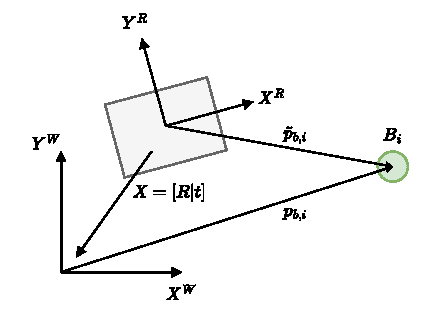
\includegraphics[width=0.8\columnwidth]{figures/localisation.pdf}}
\caption{Beacon-based Extended Kalman Filter~(EKF).}
\label{fig:localisation}
\end{figure}




\subsection{Autonomous navigation}

In the context of the Robot@Factory competition, the autonomous navigation problem can be decomposed into path planning and motion control.
Let the map representation be defined by a bi-directional graph $\mathcal{M}$ with a set of vertices $v=\{v_0,\dots,v_{j},\dots,v_{65}\}$ and a set of bi-directional edges $e=\{e_{0,1},\dots,e_{j_1,j_2},\dots,e_{26,65}\}$.
All the vertices are defined by a set of Cartesian coordinates in the global reference frame and an ID, such that $v_j=(x_j,y_j)^T$, where $j$ is the vertex ID.
For the competition, the criteria for choosing the vertices was to assign a vertex to the centre of every ArUco and keep its ID.
This option synergises with a vision-based state estimation scheme due to the fact that vertices and ArUcos share IDs, in the case of the system also using camera information for the pose estimation of the robot.
The edges were selected manually by connecting all the vertices close to each other, also taking into account the walls of the machines and warehouses on the shoop floor.
A visualisation of the graph concerning the map can be seen in Figure~\ref{fig:navigation:graph}.

\begin{figure}[!t]
\centering
\centerline{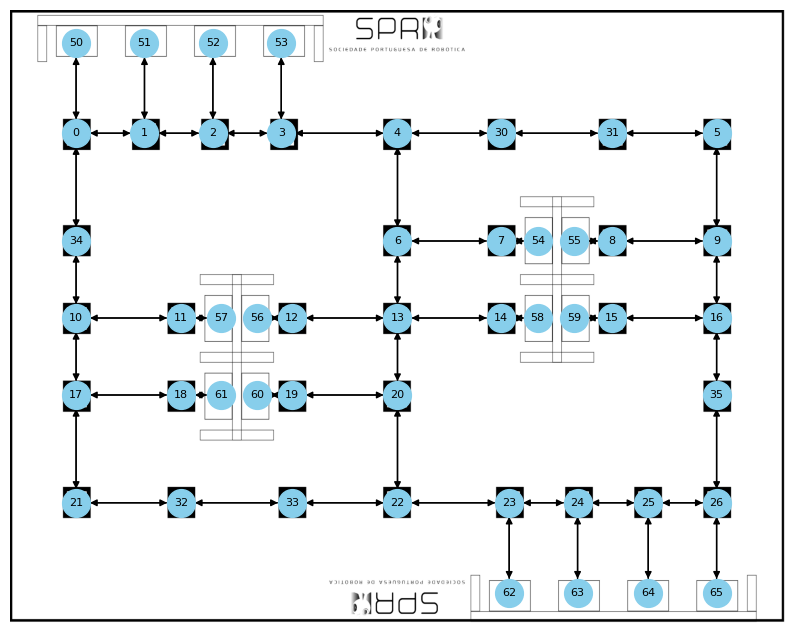
\includegraphics[width=\columnwidth]{figures/navigation-graph.png}}
\caption{Graph-based map representation of the shop floor.}
\label{fig:navigation:graph}
\end{figure}

The path planning problem is solved in this paper by using the Dijkstra graph-search algorithm~\cite{dijkstra} to find the shortest path. The starting point of the trajectory considered in the algorithm is always the vertex closest to the robot's current pose.
Then, the path planner generates the array of edges that the robot must traverse to reach its desired goal.
As for the motion control, this paper implements a line follower algorithm based on a Proportional-Integrative-Derivative~(PID) control schema to set the linear and angular reference velocities of the omnidirectional platform.
The edges from the path planner are represented as direct lines between the affected vertices of each edge.
Moreover, the error of the PID controller to set the linear velocities is formulated as the distance of the robot's current pose to the closest point in the line.
In the case of the orientation, the error is the difference between the current heading of the robot and the orientation of the last line.
This formulation is possibly due to the decoupling property between linear and angular velocity for omnidirectional robots, allowing the independent control of linear and angular velocities.



\subsection{Human-Machine Interface (HMI)}

Finally, the HMI is based on the rviz ROS visualisation tool.
First, a pre-configuration of the rviz is automatically loaded upon launching the system framework to allow the visualisation of the
ground-truth position of the beacons,
the point cloud of the 2D laser scanner,
and the robot and world coordinate frames.
Additionally, a rviz plugin was developed to add a panel to rviz, in order to allow the user to force the start of the round without requiring the communication with the UDP server handled by the competition organisers.
Lastly, the system framework also added the possibility of launching the map\_server ROS node to visualise the same shop floor shown in Figure~\ref{fig:ratf:track-2023} in rviz with the appropriate scale, to match the remaining visual data already present in rviz.





\section{Tests and Results}\label{sec:tests}

The main result of this paper is the open-source system framework available in a public GitHub repository\footref{note:repo}.
This framework includes documentation, designs, and code implementation on all the hardware, firmware, and software that led the 5dpo Robotics team to win two consecutive editions of the Robot@Factory~4.0 competition, namely, the 2022 and 2023 editions.
The framework can be used by any future participant in the competition as a development base to allow the teams to develop their own frameworks even further and study and research more advanced techniques in sensor fusion, navigation, localisation, and motion planning.
In addition to that, educators can also use this framework to foster their students' STEM education by using project-oriented learning to introduce topics related to autonomous mobile robots.

Table~\ref{tab:results:ratf} presents the final classification results for the 2022 and 2023 editions.
The table includes the three criteria mentioned in Section~\ref{sec:ratf} to rank the teams in the Robot@Factory~4.0 competition.
Although the team accomplished the same points in both editions, there is a noticeable improvement in the time taken to finish each of the three rounds of the competition, more specifically, less than half the time.
This improvement is primarily due to improved motion planning and control algorithms in the 2023 edition and the consideration of IMU data to improve the odometry estimation of the robot and, consequently, the robot's pose estimation.
The improved motion control and planning is the consideration of a graph structure in the 2023 edition, instead of a pre-defined path, and also the fact that the robot leverages the decoupling of the linear and angular velocities to rotate along the way instead of performing on-the-spot rotations.
As for the IMU, the sensor was not present in 2022, not allowing an increase in the maximum linear and angular velocities of the robot to perform the rounds faster. Note that higher velocities increase the probability of wheel slippage occurring, worsening the wheeled odometry estimation of the robot~\cite{5dpo:sousa-2022}.

\begin{table}[t!]

\centering
\caption{Final Classification Results of the 5dpo Robotics Team in the Robot@Factory~4.0 2022 and 2023 Editions.}
\label{tab:results:ratf}



\begin{tabular}{l c c c c c}

%% HEADER
\hline
\textbf{Edition} &
\textbf{Round} &
\textbf{Place} &
\textbf{\#total} &
\textbf{\#outgoing} &
\textbf{Time} (s)\\
\hline



%% TABLE CONTENTS
2022 &                  % edition
1\textsuperscript{st} & % round
1\textsuperscript{st} & % place
4                     & % #total
4                     & % #outgoing
124\\
 &                      % edition
2\textsuperscript{nd} & % round
1\textsuperscript{st} & % place
6                     & % #total
4                     & % #outgoing
126\\
 &                      % edition
3\textsuperscript{rd} & % round
1\textsuperscript{st} & % place
8                     & % #total
4                     & % #outgoing
134\\
\hline
2023 &                  % edition
1\textsuperscript{st} & % round
1\textsuperscript{st} & % place
4                     & % #total
4                     & % #outgoing
40.7\\
 &                      % edition
2\textsuperscript{nd} & % round
1\textsuperscript{st} & % place
6                     & % #total
4                     & % #outgoing
47.3\\
 &                      % edition
3\textsuperscript{rd} & % round
1\textsuperscript{st} & % place
8                     & % #total
4                     & % #outgoing
60.9\\
\hline



\end{tabular}



\end{table}


Another improvement in the 2023 edition is using the ROS framework itself.
In 2022, the software part was based on a monolithic application based in Lazarus to provide a graphical user interface to the user of the system framework, even though implementing similar methodologies to the ones presented in this paper.
The transition to C++ and ROS-based software in the 2023 participation brought the modularity inherent to separating the different modules (e.g., the EKF localiser, odometry estimation, and motion control and planning) into independent nodes, improving the maintainability and reusability of the framework by the community.

Lastly, there are videos publicly available in YouTube to show the execution of the system framework proposed in this paper. The videos include the participation in the Robot@Factory~4.0 2022\footnote{\href{https://www.youtube.com/playlist?list=PLvp8fJUEPxYR13wTYem5suJp8_--02_mJ}{https://www.youtube.com/playlist?list=PLvp8fJUEPxYR13wTYem5suJ\\p8{-}{-}02\_mJ}} and 2023\footnote{\href{https://www.youtube.com/playlist?list=PLvp8fJUEPxYT8sAByXptjetaSgl28VxxH}{https://www.youtube.com/playlist?list=PLvp8fJUEPxYT8sAByXptjetaS\\gl28VxxH}} editions.





\section{Conclusions and Future Work}\label{sec:conclusions}

In conclusion, the system framework proposed in this paper is modular and open-source to let future participants in the Robot@Factory~4.0 competition use it as their development base.
The framework modularity allows the users to modify individual modules without interfering with other ones. The public GitHub repository\footref{note:repo} has the hardware documentation and designs (including the 3D models of the robot's parts), the firmware implementation for the Arduino Mega 2560, and the ROS-based software developed in the scope of the competition, facilitating the reuse of the system framework.
Furthermore, the framework proposed in this paper may be used for academic purposes to promote the STEM education of students with a project-oriented learning approach to introduce basic robotics concepts.
As future work, the ROS~2 compatibility will be implemented for the system framework, added camera support to detect the ArUco markers and use them in the update step of the EKF localiser, and the elaboration of a STEM education activity will be considered with even further documentation and more class-oriented contents.





\section*{Acknowledgment}

In the name of the 5dpo Robotics team, the authors thank the Electrical and Computers Engineering Department~(DEEC) from the Faculty of Engineering, University of Porto~(FEUP), the faculty itself, and the INESC TEC -- Institute for Systems and Computer Engineering, Technology and Science for all their support and assistance in the development of this work.





%%%%%%%%%%%%%%%%%%%%%%
%%%%% REFERENCES %%%%%
%%%%%%%%%%%%%%%%%%%%%%

\printbibliography





\end{document}
